\documentclass{article}
\usepackage[utf8]{inputenc}
\usepackage[english]{babel}
\usepackage[]{amsthm}
\usepackage[]{amssymb}
\usepackage[]{amsmath}
\usepackage[]{graphicx}
\usepackage[]{hyperref}
\usepackage[]{xcolor}
\usepackage[]{cancel}
\usepackage[]{fancyhdr}
\hypersetup{
    colorlinks,
    linkcolor={red!50!black},
    citecolor={blue!50!black},
    urlcolor={blue!80!black}
}

\pagestyle{fancy}
\fancyhf{}
\title{\vspace{-4cm}MTH20012 - Series and Transformations Test 2}
\author{Joshua Rogers}
\lhead{MTH20012 Test 2}
\rhead{Joshua Rogers 101096819}
\date\today

\begin{document}
\maketitle 

\section*{Part A}
\subsection*{One - Two}
\subsubsection*{Answers}
See images below.
\begin{figure}
\centering
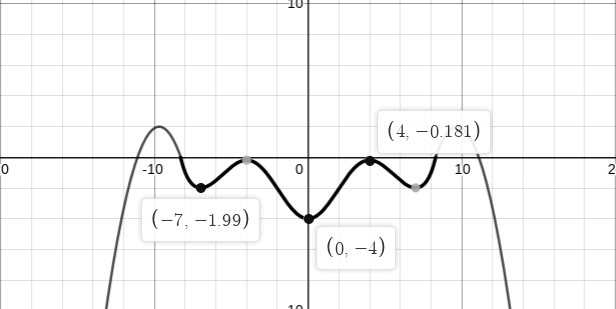
\includegraphics[width=1.0\textwidth]{./static/graph1.png}
\caption{Q1}
\end{figure}

\begin{figure}
\centering
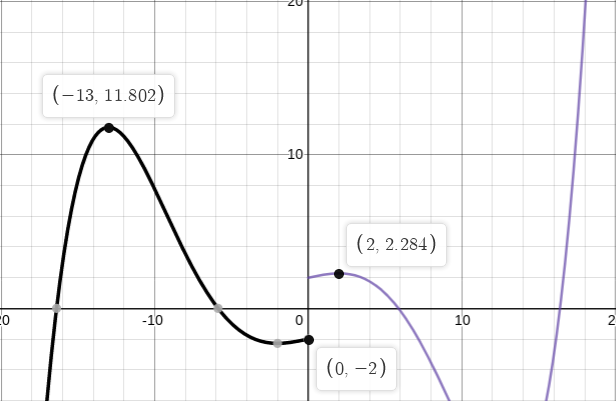
\includegraphics[width=1.0\textwidth]{./static/graph2.png}
\caption{Q2}
\end{figure}

\subsection*{Three}

Determine whether the following function is even, odd, or neither.

$$p_e\left(q_e\left(t\right)\right)r_o\left(s_o\left(t\right)\right)$$
\subsubsection*{Answers}

The composition of two even functions are even. The composition of two odd functions is odd. The product of an even function and an odd function is odd.
Thus, the answer must be an odd function.

\subsection*{Four}

Determine whether the following function is even, odd, or neither.

$$ P_o\left(Q_o\left(t\right)\right)-R_e\left(S_o\left(t\right)\right) $$

\subsubsection*{Answers}

The composition of two odd functions are odd. The composition of an even and odd function is even. The difference between an odd and even function is neither odd nor even. Thus, the function is neither odd nor even.

\end{document}
